\documentclass[10pt,english]{article}
\usepackage[T1]{fontenc}
\usepackage[latin9]{inputenc}
\usepackage{geometry}
\geometry{verbose,tmargin=1.5in,bmargin=1.5in,lmargin=1.5in,rmargin=1.5in}
\usepackage{amsthm}
\usepackage{amsmath}
\usepackage{amssymb}

\usepackage{tikz}
\makeatletter
\usepackage{enumitem}
\newlength{\lyxlabelwidth}

\usepackage[T1]{fontenc}
\usepackage{ae,aecompl}

%\usepackage{txfonts}

\usepackage{microtype}

\usepackage{calc}
\usepackage{enumitem}
\setenumerate{leftmargin=!,labelindent=0pt,itemindent=0em,labelwidth=\widthof{\ref{last-item}}}

\makeatother

\usepackage{babel}
\begin{document}
\noindent \begin{center}
\textbf{\large{}MATH 239 - Assignment 7}\\
\textbf{\large{}Chris Ji 20725415}
\par\end{center}{\large \par}
\medskip{}

\begin{enumerate}
\item \begin{enumerate}
    \item \leavevmode\vadjust{\vspace{-\baselineskip}}\newline
    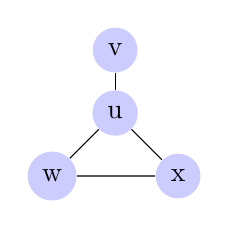
\begin{tikzpicture}
  [scale=.8,auto=left,every node/.style={circle,fill=blue!20},baseline]
  \node (n1) at (0,0)   {u};
  \node (n2) at (-1,-1)   {w};
  \node (n3) at (1,-1)    {x};
  \node (n4) at (0,1)    {v};
  \foreach \from/\to in {n1/n2,n1/n3,n2/n3,n1/n4}
    \draw (\from) -- (\to);
    
\end{tikzpicture} \\ 
For the above graph, note that there is an even length path $(u,w,x,u,v)$, however there is no even length walk from $u$ to $v$. This will be true for any graph with an odd length cycle, and then an odd length path originating from a vertex in the cycle. This is because you can always get an even length walk by walking through the cycle (odd number), and then walking down the path (+ odd number=even number), but to get the corresponding path to that walk, you can't traverse the cycle (as all walks from $(u\ldots u)$ are just replaced by a single u), so the path must be an odd length. 

    \item \leavevmode\vadjust{\vspace{-\baselineskip}}\newline
    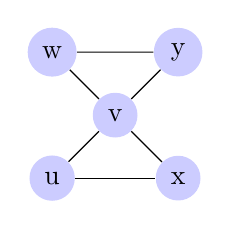
\begin{tikzpicture}
  [scale=.8,auto=left,every node/.style={circle,fill=blue!20},baseline]
  \node (n1) at (0,0)   {v};
  \node (n2) at (-1,-1)   {u};
  \node (n3) at (1,-1)    {x};
  \node (n4) at (1,1)    {y};
  \node (n5) at (-1,1)    {w};
  \foreach \from/\to in {n1/n2,n1/n3,n2/n3,n1/n4,n1/n5,n4/n5}
    \draw (\from) -- (\to);
\end{tikzpicture} \\ 
There is clearly a cycle containing $u,v$ and $v,w$, and no cycle containing $u,w$. This will be true for any graph containing cycles with $u,v$ and $v,w$ such that any path from $u,w$ has to go through $v$ ($v$ is like a vertex bridge). This is because if $v$ is the only bridge, then there is no way to create more than one $u,w$ path, so there can't be a cycle containing $u,w$. 

\end{enumerate}

\pagebreak
\item Partition $G$ into $A,B$ and $H$ into $C,D$ such that $|A|,|B|,|C|,|D|\geq1$, and so that there are no edges connecting any vertex in $A$ to $B$, and there are no edges connecting any vertex in $C$ to $D$. Furthermore, represent $V(G)=\{v_0,\ldots,v_k,v_{k+1},\ldots,v_n\}$, such that there are no edges connecting $\{v_0,\ldots,v_k\}$ to $\{v_{k+1},\ldots,v_n\}$ (either $v_i\in A$ for all $i\leq k$, or $v_i\in B$ for all $i\leq k$). Represent $V(H)$ similarly by $\{w_0,\ldots,w_l,w_{l+1},\ldots,w_n\}$. Note that $A$ must share at least one vertex, say $v$, with either $C$ or $D$, as we have completely partitioned $G$ and $H$. As order doesn't matter in our partitions, set $v_0=w_0=v$. By similar logic, $B$ must share at least one vertex, say $w$, with the other set (if $v$ is in $A$ and $C$, then $w$ is in $B$ and $D$, and if $v$ is in $A$ and $D$, then $w$ is in $B$ and $C$), and so set $v_n=w_n=w$. Then we can see that $v,w\in V(G)$ are in different components in both $G$ and $H$.

\pagebreak
\item Lets look at a subgraph of $G$, $H$, that is the component of $G$ that contains $u,v$. Since all vertices other than $u,v$ have even degree, then all other components are cycles, and hence have no bridges (and we do not care about them). Note every vertex in $H$ other than $u,v$ has even degree, and least $2$ neighbours (since $H$ is connected). If an edge $e$ is a bridge of $G$, then there are no cycles containing $e$. Let's induct on the length of the shortest $uv-$path. If the length is $1$, then clearly either the edge $\{u,v\}$ is a bridge, or $H$ (and therefore $G$) has no bridges, as then $u,v$ must be in the same cycle, and all other vertices are also in a cycle since they have degree at least 2. Now that $P=(u,u_{1},\ldots,u_{n-1},v)$. If $u$ and $v$ are both degree 1, then $\{u,u_{1}\}$ and $\{u_{n-1},v\}$ are both bridges, and they are clearly contained in our path. Furthermore, if every $u_i$ has degree 2, then every $\{u_{i},u_{i+1}\}$ is a bridge, and is contained in our path. Else, some $u_j$ has degree $>2$, and so if we remove all of the vertices after the last $u_j$ with degree $>2$, we have that this subgraph has at least one cycle (since all the vertices other than $u$ have degree at least 2). Then every edge after $u_j$ is a bridge (since it isn't in a cycle), and is contained in our path. Similarly, if we take $u_j$ such that $j$ is minimized, we can remove all of the vertices before the first $u_k$ with degree $>2$, and we can see that all $u_i$ such that $i<j$ is a bridge, since there is a cycle containing the $u_i$'s after $u_j$. Then this path contains all the bridges of $H$, and hence $G$. Note that while this is only the shortest path, any other path is just traversing the other way around any cycles, and will have to pass through the same bridges. 


\pagebreak
\item \begin{enumerate}
    \item Assume that $G$ has no cycles. Take $P=(v_0,v_1\ldots,v_n)$ to be the longest path in $G$. Then the final vertex in the path, $v_n$, must have $k-1$ edges that are not connected to any vertex already in the path, or else it would be a cycle. This contradicts our earlier assumption that $P$ is the longest path. So then each one of the $k-1$ edges must connect to a vertex in our path. Let $v_i$ be the vertex in $P$ that connects to $v_n$ such that there is no smaller index $i$ of $v$ in our path. Then there is a cycle $(v_i,\ldots,v_n,v_i)$, and since there are at least $k-1$ vertices between $v_i$ and $v_n$, the cycle is at least of length $k+1$. 
    \item Assume that $G$ only has odd length cycles. Take $P=(v_0,v_1,\ldots,v_n)$ to be the longest path in $G$. But since $v_n$ has at least 3 neighbours, it must be connected to two different cycles, $C_1=(w_0,\ldots,v_n,w_0)$ and $C_2=(y_0,\ldots,v_n,y_0)$ that share an edge ($v_n$ can not be the bridge between two cycles, as then it would not be the final vertex in a longest path), say, $\{w_i,y_j\}$, and clearly both contain $v_n$. Since $C_1$ and $C_2$ are both odd length, the cycle $(w_0,v_n,\ldots,w_0,\ldots,w_i,\ldots,w_0)$ is of even length. 
\end{enumerate}

\pagebreak
\item If a graph $G=(V,E)$ has $|V(G)|=n$ vertices, then by handshake lemma, \begin{align*}\sum_{v\in V}\text{deg}(v)&=2|E(G)|\\\Rightarrow k*1+(n-k)*3&=2|E(G)|\\\Rightarrow 3n-2k&=2|E(G)|\\\Rightarrow |E(G)|&=\frac{3n-2k}{2}\end{align*} This is because there are $k$ vertices with degree 1, and $n-k$ vertices with degree 3. Note that from the question we know that \begin{align*}|E(G)|&=|V(G)|+\alpha\\\Rightarrow |E(G)|=n+\alpha&=\frac{3n-2k}{2}\\\Rightarrow 2n+2\alpha&=3n-2k\\\Rightarrow 2\alpha&=n-2k\\\Rightarrow n&=2k+2\alpha\end{align*} as required.


\end{enumerate}

\end{document}
